

\tikzset{every picture/.style={line width=0.75pt}} %set default line width to 0.75pt        

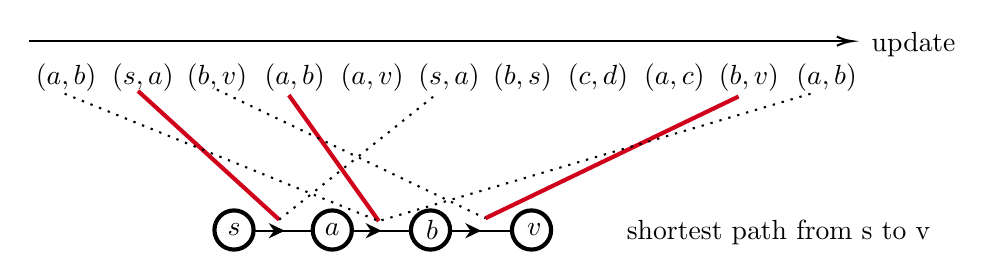
\begin{tikzpicture}[x=0.5pt,y=0.5pt,yscale=-1,xscale=1]
%uncomment if require: \path (0,193); %set diagram left start at 0, and has height of 193

%Straight Lines [id:da42563372855460047] 
\draw [color={rgb, 255:red, 0; green, 0; blue, 0 }  ,draw opacity=1 ][line width=0.75]    (253.5,160) -- (296.5,160) ;
\draw [shift={(275,160)}, rotate = 180] [fill={rgb, 255:red, 0; green, 0; blue, 0 }  ,fill opacity=1 ][line width=0.08]  [draw opacity=0] (11.61,-5.58) -- (0,0) -- (11.61,5.58) -- (7.71,0) -- cycle    ;
%Straight Lines [id:da13574797376852343] 
\draw [color={rgb, 255:red, 0; green, 0; blue, 0 }  ,draw opacity=1 ][line width=0.75]    (325.5,160) -- (368.5,160) ;
\draw [shift={(347,160)}, rotate = 180] [fill={rgb, 255:red, 0; green, 0; blue, 0 }  ,fill opacity=1 ][line width=0.08]  [draw opacity=0] (11.61,-5.58) -- (0,0) -- (11.61,5.58) -- (7.71,0) -- cycle    ;
%Straight Lines [id:da9930965641121888] 
\draw    (20,23) -- (613,23) ;
\draw [shift={(615,23)}, rotate = 180] [color={rgb, 255:red, 0; green, 0; blue, 0 }  ][line width=0.75]    (10.93,-3.29) .. controls (6.95,-1.4) and (3.31,-0.3) .. (0,0) .. controls (3.31,0.3) and (6.95,1.4) .. (10.93,3.29)   ;
%Straight Lines [id:da09874107164515367] 
\draw [color={rgb, 255:red, 0; green, 0; blue, 0 }  ,draw opacity=1 ][line width=0.75]    (183.5,160) -- (226.5,160) ;
\draw [shift={(205,160)}, rotate = 180] [fill={rgb, 255:red, 0; green, 0; blue, 0 }  ,fill opacity=1 ][line width=0.08]  [draw opacity=0] (11.61,-5.58) -- (0,0) -- (11.61,5.58) -- (7.71,0) -- cycle    ;
%Straight Lines [id:da6519777460675502] 
\draw [color={rgb, 255:red, 208; green, 2; blue, 27 }  ,draw opacity=1 ][line width=1.5]    (201,152) -- (99,59) ;
%Straight Lines [id:da29298485524387174] 
\draw [color={rgb, 255:red, 208; green, 2; blue, 27 }  ,draw opacity=1 ][line width=1.5]    (273,153) -- (208,62) ;
%Straight Lines [id:da3208602618624562] 
\draw [color={rgb, 255:red, 208; green, 2; blue, 27 }  ,draw opacity=1 ][line width=1.5]    (350,151) -- (533,63) ;
%Straight Lines [id:da419202195721033] 
\draw  [dash pattern={on 0.84pt off 2.51pt}]  (46,61) -- (273,153) ;
%Straight Lines [id:da11015742569478726] 
\draw  [dash pattern={on 0.84pt off 2.51pt}]  (585,61) -- (273,153) ;
%Straight Lines [id:da5872263776878417] 
\draw  [dash pattern={on 0.84pt off 2.51pt}]  (201,152) -- (315,61) ;
%Straight Lines [id:da26779689112701766] 
\draw  [dash pattern={on 0.84pt off 2.51pt}]  (156,58) -- (350,151) ;

% Text Node
\draw  [line width=1.5]   (168.38, 159.47) circle [x radius= 14.15, y radius= 14.15]   ;
\draw (168.38,159.47) node   [align=left] {$\displaystyle s$};
% Text Node
\draw  [line width=1.5]   (239.38, 159.47) circle [x radius= 14.15, y radius= 14.15]   ;
\draw (239.38,159.47) node   [align=left] {$\displaystyle a$};
% Text Node
\draw  [line width=1.5]   (310.38, 159.47) circle [x radius= 14.15, y radius= 14.15]   ;
\draw (304.88,159.47) node [anchor=west] [inner sep=0.75pt]   [align=left] {$\displaystyle b$};
% Text Node
\draw  [line width=1.5]   (383.38, 159.47) circle [x radius= 14.15, y radius= 14.15]   ;
\draw (377.88,159.47) node [anchor=west] [inner sep=0.75pt]   [align=left] {$\displaystyle v$};
% Text Node
\draw (78.06,37) node [anchor=north west][inner sep=0.75pt]   [align=left] {$\displaystyle ( s,a)$};
% Text Node
\draw (572.6,37) node [anchor=north west][inner sep=0.75pt]   [align=left] {$\displaystyle ( a,b)$};
% Text Node
\draw (243.24,37) node [anchor=north west][inner sep=0.75pt]   [align=left] {$\displaystyle ( a,v)$};
% Text Node
\draw (132.12,37) node [anchor=north west][inner sep=0.75pt]   [align=left] {$\displaystyle ( b,v)$};
% Text Node
\draw (188.18,37) node [anchor=north west][inner sep=0.75pt]   [align=left] {$\displaystyle ( a,b)$};
% Text Node
\draw (407.42,37) node [anchor=north west][inner sep=0.75pt]   [align=left] {$\displaystyle ( c,d)$};
% Text Node
\draw (462.48,37) node [anchor=north west][inner sep=0.75pt]   [align=left] {$\displaystyle ( a,c)$};
% Text Node
\draw (299.3,37) node [anchor=north west][inner sep=0.75pt]   [align=left] {$\displaystyle ( s,a)$};
% Text Node
\draw (353.36,37) node [anchor=north west][inner sep=0.75pt]   [align=left] {$\displaystyle ( b,s)$};
% Text Node
\draw (627,14) node [anchor=north west][inner sep=0.75pt]   [align=left] {update};
% Text Node
\draw (23,37) node [anchor=north west][inner sep=0.75pt]   [align=left] {$\displaystyle ( a,b)$};
% Text Node
\draw (516.54,37) node [anchor=north west][inner sep=0.75pt]   [align=left] {$\displaystyle ( b,v)$};
% Text Node
\draw (450,150) node [anchor=north west][inner sep=0.75pt]   [align=left] {shortest path from s to v};


\end{tikzpicture}

